\section{L8}

接著 L7 的 MAC。


\subsection{MAC}


\paragraph{Security of Fixed-length MAC}

\begin{theorem}
	If \(F\) is PRF, then \(\Pi\) is existentially unforgeable under adaptive chosen message attack (in \(\MacForge\) experiment).
\end{theorem}

\begin{myProof}[Security proof of PRF-based construction]
	Consider \(\widetilde{\Pi} = (\widetilde{\Gen}, \widetilde{\Mac}, \widetilde{\Vrfy})\) constructed by the random function. \\
	Then we know that \(\Pr[\MacForge_{A, \widetilde{\Pi}}(n) = 1] \leq 2^{-n}\) \\
	because for any \(m \not\in Q\), the tag \(t = f(m)\) is uniformly distributed in \(\{0, 1\}^n\) from \(A\)'s view.
	
	Our goal of proof:
	\begin{align*}
		&| \Pr[\MacForge_{A, \Pi}(n) = 1] - \Pr[\MacForge_{A, \widetilde{\Pi}}(n) = 1] | \leq \negl(n) \\
		\Rightarrow \quad &\Pr[\MacForge_{A, \Pi}(n) = 1] \leq 2^{-n} + \negl(n) \\
		\Rightarrow \quad &\Pr[\MacForge_{A, \Pi}(n) = 1] \leq \negl(n)
	\end{align*}
	
	We then contruct a distringuisher \(D\) who want to break PRF security. \(D\) can do oracle access to some functions, and finally determines such function is pseudorandom (i.e. \(F_k\) for uniform \(k \in \{0, 1\}^n\)) or truly random (i.e. \(f\) for uniform \(f \in \Func_n\)).
	
	Reduction:
	\begin{center}
		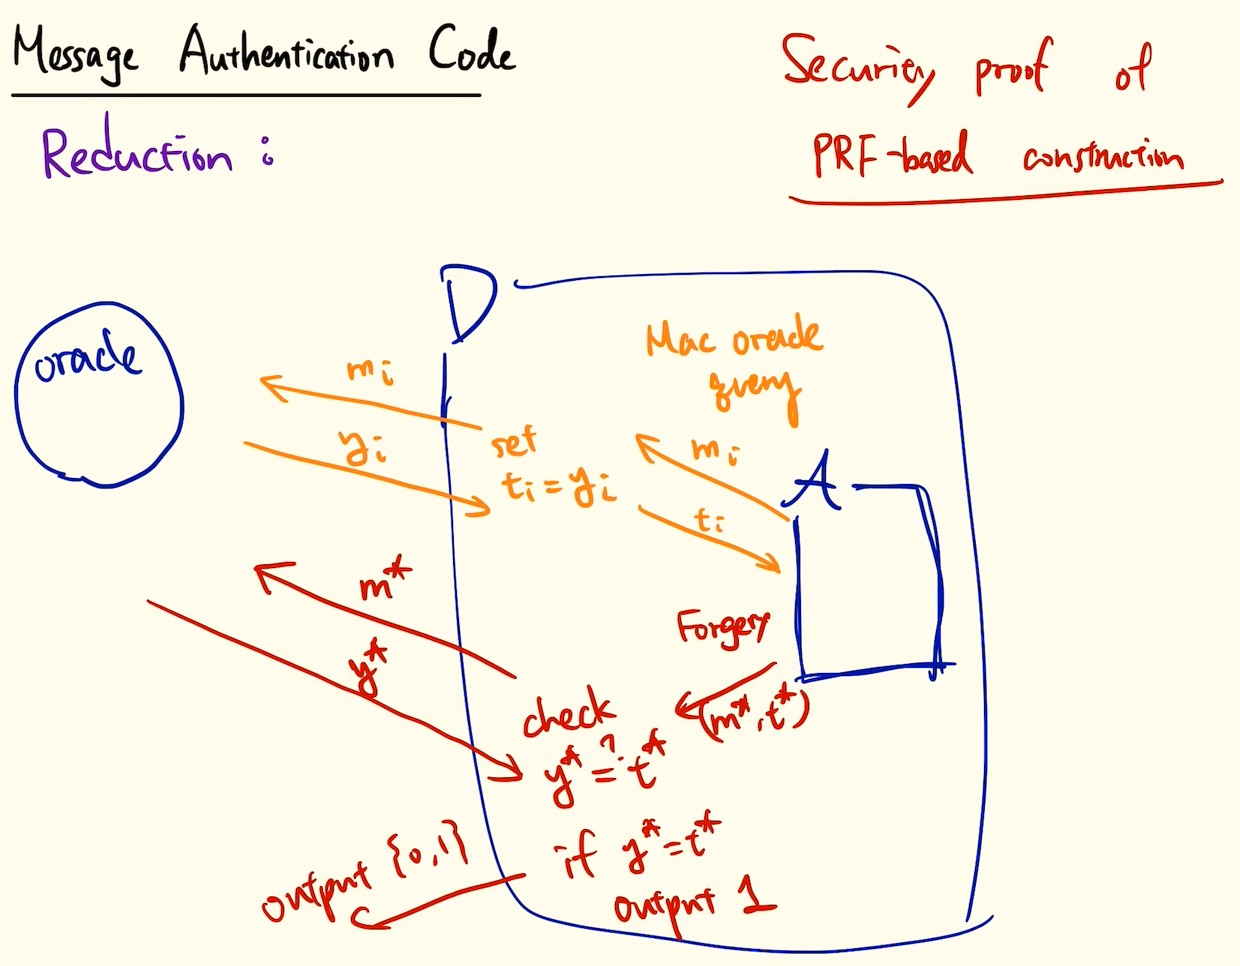
\includegraphics[width=0.7\textwidth, keepaspectratio]{MacForge_reduction.jpg}
	\end{center}
	
	\begin{enumerate}[label=(\roman*)]
		\item If \(D\)'s oracle is PRF,
			\[\Pr[D^{F_k(\cdot)}(1^n) = 1] = \Pr[\MacForge_{A, \Pi}(1^n) = 1]\]
		\item If \(D\)'s oracle is random function,
			\[\Pr[D^{f(\cdot)}(1^n) = 1] = \Pr[\MacForge_{A, \widetilde{\Pi}}(n) = 1] \leq 2^{-n}\]
		\item If By assumption,
			\[ |\Pr[D^{F_k(\cdot)}(1^n) = 1] - \Pr[D^{f(\cdot)}(1^n) = 1]| \leq \negl(n)\]
	\end{enumerate}
	綜合上面三點,
	\[ \Pr[\MacForge_{A, \Pi}(n) = 1] \quad \leq 2^{-n} + \negl(n) \quad \leq \negl(n) \]
	
\end{myProof}

\subparagraph{Quiz}

Say \(\Pi = (\Gen, \Mac, \Vrfy)\) is a MAC with tag size \(t(n)\). \\
Show that if \(t(n) = O(\log(n))\), then \(\Pi\) is not secure MAC. \\
(Hint: PPT adversary runs \textbf{random guess})


\paragraph{MAC for Arbitrary-length Messages (domain extension of MAC)}

Let \(\Pi' = (\Gen', \Mac', \Vrfy')\) be a fixed-length MAC for message size \(n\), and \(\Pi = (\Gen, \Mac, \Vrfy)\) is a MAC for arbitrary-length messages.

\begin{itemize}[itemsep=10pt]
	\item \(\Gen\): identical to \(\Gen'(1^n) \rightarrow k\), where \(k \in \{0, 1\}^n\)
	
	\item \(\Mac\): on input \(k \in \{0, 1\}^n\) and a message \(\{0, 1\}^*\) of length \(l < \frac{n}{4}.\)
		\begin{enumerate}[label=(\roman*)]
			\item Parse \(m\) into \(d\) blocks \(m_1, m_2, \ldots, m_d\) (each of length \(\frac{n}{4}\)). \\
			The final block is padded with \(0\)s.
			\item choose a uniform \(r \in \{0, 1\}^{\frac{n}{4}}\)
			\item For \(i = 1, 2, \ldots, d\), compute \(t_i \leftarrow \Mac'_k(r \, || \, l \, || \, i \, || \, m_i)\) where all the length of \(r, l, i, m\) are \(\frac{n}{4}\) bits respectively.
			\item Output \(t = (r, t_1, t_2, \ldots, t_d)\).
		\end{enumerate}

	\item \(\Vrfy\): On input \(k, t, m\),
		\begin{enumerate}[label=(\roman*)]
			\item Parse \(m\) and \(t\), such that \(m = (m_1, m_2, \ldots, m_d)\) and \(t = (r, t_1, t_2, \ldots, t_{d'})\).
			\item Output 1 if the below are both satisfied:
			\begin{itemize}
				\item \(d' = d\)
				\item For \(1 \leq i \leq d\), \(\Vrfy'(r \, || \, l \, || \, i \, || \, m_i) = 1\).
			\end{itemize}
		\end{enumerate}
\end{itemize}

\subparagraph{Remark of \(\Mac\)}

It seems \(r, l, i\) are important for security.

如果 \(\Mac'\) 中沒有 \(l\),則 \(t_i \leftarrow \Mac'_k(r \, || \, i \, || \, m_i \, || 0^{\frac{n}{4}})\)。 \\
此時 adversary 的可以這樣進行攻擊:
\begin{steps}
	\item 選取一個 \(m\) 來詢問 MAC oracle,並從 MAC oracle 收到 \(t = (r, t_1, \ldots, t_d)\)
	\item 偽造 \(m^\ast = (m_1, m_2, \ldots, m_{d-1})\) 和 \(t^\ast = (r, t_1, t_2, \ldots, t_{d-1})\)。
\end{steps}

由於 \(m^\ast\) 之前並沒有被拿來問 MAC oracle,所以 adversary 是成功的。

這說明 \(l\) 是重要的。

\subparagraph{Quiz}

In domain extension of MAC, it is in secure if there is no \(r\) or \(i\).
\begin{myEnumerate}[label=(\arabic*)]
	\item Show an attack if no \(r\).
	\item Show an attack if no \(i\).
\end{myEnumerate}

\begin{theorem}
	If MAC for fixed length \(\Pi'\) is secure, then MAC for arbitrary length \(\Pi\) is secure.
\end{theorem}


\paragraph{CBC-MAC}

每個 block 計算完後就跟下一個 block 做 xor 再繼續計算,最終只會得到一個 tag \(t\)。

\begin{center}
	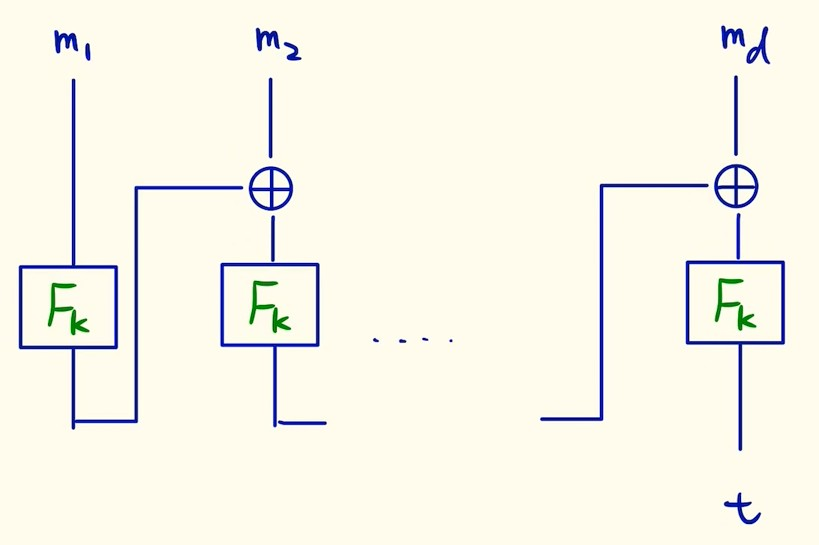
\includegraphics[width=0.5\textwidth, keepaspectratio]{CBC-MAC.jpg}
\end{center}

\subparagraph{Quiz}

Analyze advantages and disadvantages of CBC-MAC and domain extension. \\ 
(Hint: compare in performance, security, adjustment of parameters, etc.)
